\documentclass[a4paper]{article}

\usepackage[UTF8]{ctex}
\usepackage[a4paper,margin=1in]{geometry}
\usepackage{graphicx}
\usepackage{float}
\usepackage{listings}
% \usepackage{listings-rust}
\usepackage{longtable}
\usepackage{booktabs}
\usepackage{hyperref}
\usepackage{fancyhdr}
\usepackage{lastpage}
\usepackage{color}
\usepackage{indentfirst}        % 首段缩进
\setlength{\parindent}{2em}     % 缩进2字符
\usepackage{zhnumber}           % 中文编号
\usepackage[dvipsnames,table,xcdraw]{xcolor}
\usepackage{adjustbox}
\usepackage{subcaption}
\usepackage{amsmath}
\usepackage{amssymb}
\usepackage[many]{tcolorbox}
% \newfontfamily{\enfont}{Arial}  % 定义英文字体
\usepackage{enumitem}
\usepackage{xeCJK}
\usepackage[T1]{fontenc}
\usepackage{lmodern}
\usepackage{inconsolata} % 使用更美观的等宽字体 Inconsolata
\usepackage{multirow} % 用于表格中的多行合并
\usepackage{tikz} % 添加 TikZ 宏包用于绘制流程图
\usetikzlibrary{positioning} % 添加定位库以支持 'of' 语法
\usepackage{array} % 提供 >{...} 列类型支持（修复表格中 \arraybackslash 的用法）

% 全局设置（影响所有级别）
\setlist[itemize]{
    itemsep=2pt,
    topsep=4pt,
    parsep=1pt,
    leftmargin=3em
}

% 仅设置第一级（最高级）
\setlist[itemize,1]{
    label=\textcolor{orange}{$\blacktriangleright$},
    font=\color{blue!80!black}\small\bfseries,
    before={\color{blue!80!black}\small\bfseries}
}

% 重置第二级及更深级别（恢复默认样式）
\setlist[itemize,2]{
    label={\normalfont\textbullet},
    font=\normalfont\normalsize\color{black},
    before={\color{black}},
    leftmargin=*
}
\setlist[itemize,3]{
    label={\normalfont$\circ$},
    font=\normalfont\normalsize,
    before={},
    leftmargin=*
}


% 定义可分页的引用环境
\newtcolorbox[auto counter]{myquote}[1][]{
    % breakable,                     % 允许跨页分断
    % enhanced jigsaw,               % 优化分页处的边框
    colback=gray!5,                % 背景色
    colframe=gray!30,              % 边框色
    left=5mm, right=5mm,           % 左右内边距
    top=3mm, bottom=3mm,           % 上下内边距
    width=0.85\textwidth,         % 宽度
    center,                     % 居中
    arc=0mm,                       % 直角边框
    boxrule=0.5pt,                 % 边框线宽
    fontupper=\small\linespread{1.1}\selectfont, % 行距微调（1.1倍）
    % fontupper=\sffamily\linespread{1.05}\selectfont, % 无衬线 + 紧凑行距
    before upper={\parindent2em\color{black!40!blue}\itshape\small\kaishu}, % 深蓝色文本
    #1 % 允许额外参数
}

%\newcommand{\college}{中山大学计算机学院}
\newcommand{\projname}{计算机网络实验|实验八}
\newcommand{\reporttitle}{快速生成树协议配置}
\newcommand{\groupno}{第一组}
\newcommand{\authorname}{欧阳易芃、马福泉、刘昊、彭怡萱}
\newcommand{\major}{计算机科学与技术}
\newcommand{\adviser}{谢逸}
\newcommand{\startdate}{2025年12月7日}
\newcommand{\labenddate}{2025年12月20日}
\newcommand{\labroom}{实验D402}

\pagestyle{fancy} % 使用 fancyhdr 风格
\fancyhf{}      % 清空默认的页眉页脚

% 设置页眉
\fancyhead[L]{\kaishu \projname}      % 左侧页眉显示项目名称
\fancyhead[C]{\kaishu \reporttitle}    % 中间页眉显示报告标题
\fancyhead[R]{\kaishu \authorname} % 右侧页眉显示作者姓名

% 设置页脚
\fancyfoot[C]{第 \thepage 页，共 \pageref{LastPage} 页} % 中间页脚显示页码

% 去除页眉页脚与正文之间的分隔线
\renewcommand{\headrulewidth}{0.4pt}
\renewcommand{\footrulewidth}{0pt}

% 设置文档背景颜色
\definecolor{mybgcolor}{RGB}{0, 0, 0} % 定义背景颜色
\definecolor{NavyBlue}{RGB}{0,0,128} % 添加颜色定义



% 全局设置lstlisting的样式
\lstset{
    language=C, % 设置默认语言
    basicstyle=\footnotesize\ttfamily, % 设置字体族
    breaklines=true, % 自动换行
    keywordstyle=\bfseries\color{blue}, % 设置关键字为粗体，颜色为蓝色
    morekeywords={}, % 设置更多的关键字，用逗号分隔
    emph={}, % 指定强调词，如果有多个，用逗号隔开
    emphstyle=\bfseries\color{Rhodamine},
    commentstyle=\itshape\color{green!50!black},
    stringstyle=\bfseries\color{PineGreen!90!black},
    columns=fullflexible,% 设置列宽
    numbers=left,
    numbersep=2em,
    numberstyle=\footnotesize\color{gray},
    frame=single,
    framesep=1em,
    showstringspaces=false,% % 不显示字符串中的空格
    keepspaces=true,
    backgroundcolor=\color{gray!5},
    % linewidth=0.8\linewidth, % 设置宽度为当前行宽的 80%
    xleftmargin=0.2\linewidth, % 左右边距自动调整
    xrightmargin=0.08\linewidth,
    % gobble=2, % 可选：移除代码前的缩进
    % postbreak=\mbox{\textcolor{red}{$\hookrightarrow$}\space}, % 可选：换行符样式
    captionpos=b, % 可选：标题位置
    aboveskip=1em, % 可选：上方间距
    belowskip=1em, % 可选：下方间距
}

\begin{document}


% 封面
\begin{titlepage}
    \centering
    
\includegraphics[width=10cm]{img/SYSULogo.png}
    \vspace{1em}
    %{\Large \college \par}
    \vspace{1em}
    \makebox[\textwidth][c]{\Large \kaishu \projname \par} % 项目名称居中
    \vspace{3em}
    {\fontsize{40pt}{42pt}\kaishu \selectfont \boldmath \reporttitle\par}
    \vspace*{\fill}
    \begin{center}
    {\Large
    \makebox[5em][s]{小组编号}:\underline{\makebox[15em][c]{\kaishu \groupno}}\\[1em]
    \makebox[5em][s]{组员姓名}:\underline{\makebox[15em][c]{\kaishu 欧阳易芃、马福泉}}\\[0.5em]
    \makebox[5em][s]{} \underline{\makebox[15em][c]{\kaishu 刘昊、彭怡萱}}\\[1em]
    \makebox[5em][s]{专业}:\underline{\makebox[15em][c]{\kaishu \major}}\\[1em]
    \makebox[5em][s]{课程教师}:\underline{\makebox[15em][c]{\kaishu \adviser}}\\[1em]
    \makebox[5em][s]{起始日期}:\underline{\makebox[15em][c]{\kaishu \startdate}}\\[1em]
    \makebox[5em][s]{结束日期}:\underline{\makebox[15em][c]{\kaishu \labenddate}}\\[1em]
    \makebox[5em][s]{实验地点}:\underline{\makebox[15em][c]{\kaishu \labroom}}
    }
    \end{center}
    \vspace*{\fill}
\end{titlepage}

% 目录
\tableofcontents
\newpage

\section{实验概述}

% 实验拓扑与环境
\paragraph{实验拓扑与环境}
\begin{itemize}
    \item \textbf{实验拓扑图：}
    \begin{figure}[H]
        \centering
        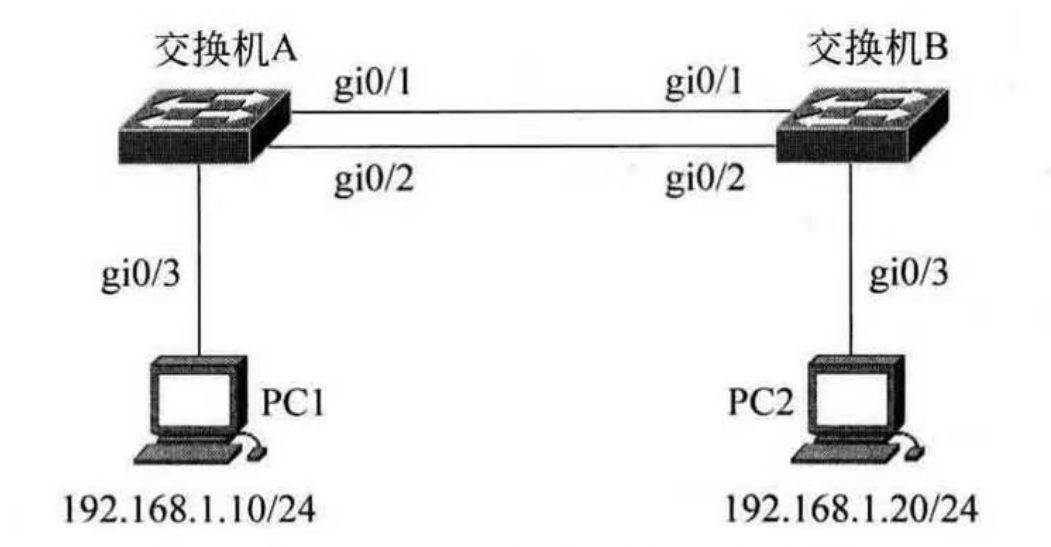
\includegraphics[width=0.7\textwidth]{img/tuopu.png}
        \caption{实验拓扑图}
    \end{figure}
    \item \textbf{设备：}
    \begin{itemize}
        \item SwitchA: 华为S5720交换机 (172.16.[X].201)
        \item SwitchB: 华为S5720交换机 (172.16.[X].202)
    \end{itemize}
    \item \textbf{VLAN规划：} VLAN 10
    \item \textbf{端口规划：}
    \begin{itemize}
        \item G0/0/3: Access端口，接入终端设备
        \item G0/0/1-2: Trunk端口，交换机间互联
    \end{itemize}
\end{itemize}

本实验围绕生成树协议（STP）及其快速版本（RSTP）的配置与分析展开，主要内容包括：
\begin{itemize}
    \item 配置快速生成树协议（RSTP），并回答实验相关问题及实验思考。
    \item 抓取生成树协议相关的数据包，分析桥协议数据单元（BPDU）的结构与内容。
    \item 在实验设备上查看VLAN生成树状态，并掌握查看其它相关重要信息的方法。
\end{itemize}

\section{理论知识}

\subsection{生成树协议（STP/RSTP）作用}
在二层以太网中，物理冗余链路易导致广播风暴、MAC地址表震荡等问题。生成树协议（STP/RSTP）通过阻塞部分端口，构建无环路的逻辑拓扑，保障网络高可用性，并在链路故障时自动激活备用路径。

\subsection{STP（802.1D）基本原理}

\begin{itemize}
    \item \textbf{根桥选举}：比较所有交换机的桥ID（优先级+MAC），值最小者为根桥。
    \item \textbf{根端口选举}：每台非根桥选择一条到根桥路径开销最小的端口作为根端口。
    \item \textbf{指定端口选举}：每个网段选出一台到根桥路径最优的交换机的端口为指定端口。根桥所有端口均为指定端口。
    \item \textbf{阻塞端口}：既非根端口也非指定端口的端口被阻塞，防止环路。
\end{itemize}

\subsection{RSTP（802.1w）主要改进}

\begin{table}[H]
    \centering
    \begin{tabular}{|p{3cm}|p{4cm}|p{4cm}|}
        \hline
        \textbf{特性} & \textbf{STP (802.1D)} & \textbf{RSTP (802.1w)} \\
        \hline
        端口角色 & 根端口、指定端口、阻塞端口 & 新增备用端口、备份端口，角色更细化 \\
        \hline
        端口状态 & 5种（禁用、阻塞、监听、学习、转发） & 3种（丢弃、学习、转发） \\
        \hline
        收敛机制 & 依赖定时器，收敛慢（30-50秒） & P/A握手机制、边缘端口，收敛快（1-2秒） \\
        \hline
        收敛速度 & 慢 & 快 \\
        \hline
    \end{tabular}
    \caption{STP与RSTP主要区别}
\end{table}

\section{实验步骤与结果}

\subsection{步骤一：初始网络状态测试}

\subsubsection{为PC1、PC2配置IP地址}

按照实验拓扑连接所有设备，为PC1和PC2分别配置静态IP地址，确保两台主机处于同一网段。

\begin{figure}[H]
    \centering
    \begin{subfigure}[b]{0.45\textwidth}
        \centering
        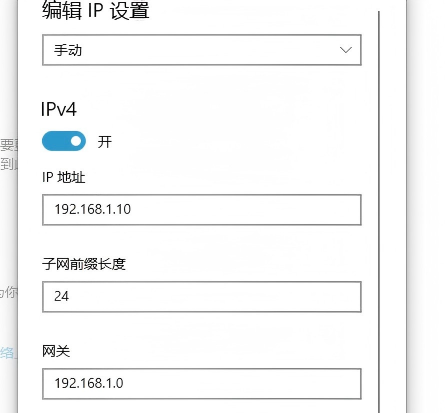
\includegraphics[width=\textwidth]{img/step1/PC1_IP_config.png}
        \caption{PC1的IP地址配置界面}
        \label{fig:PC1_IP_config}
    \end{subfigure}
    \hfill
    \begin{subfigure}[b]{0.45\textwidth}
        \centering
        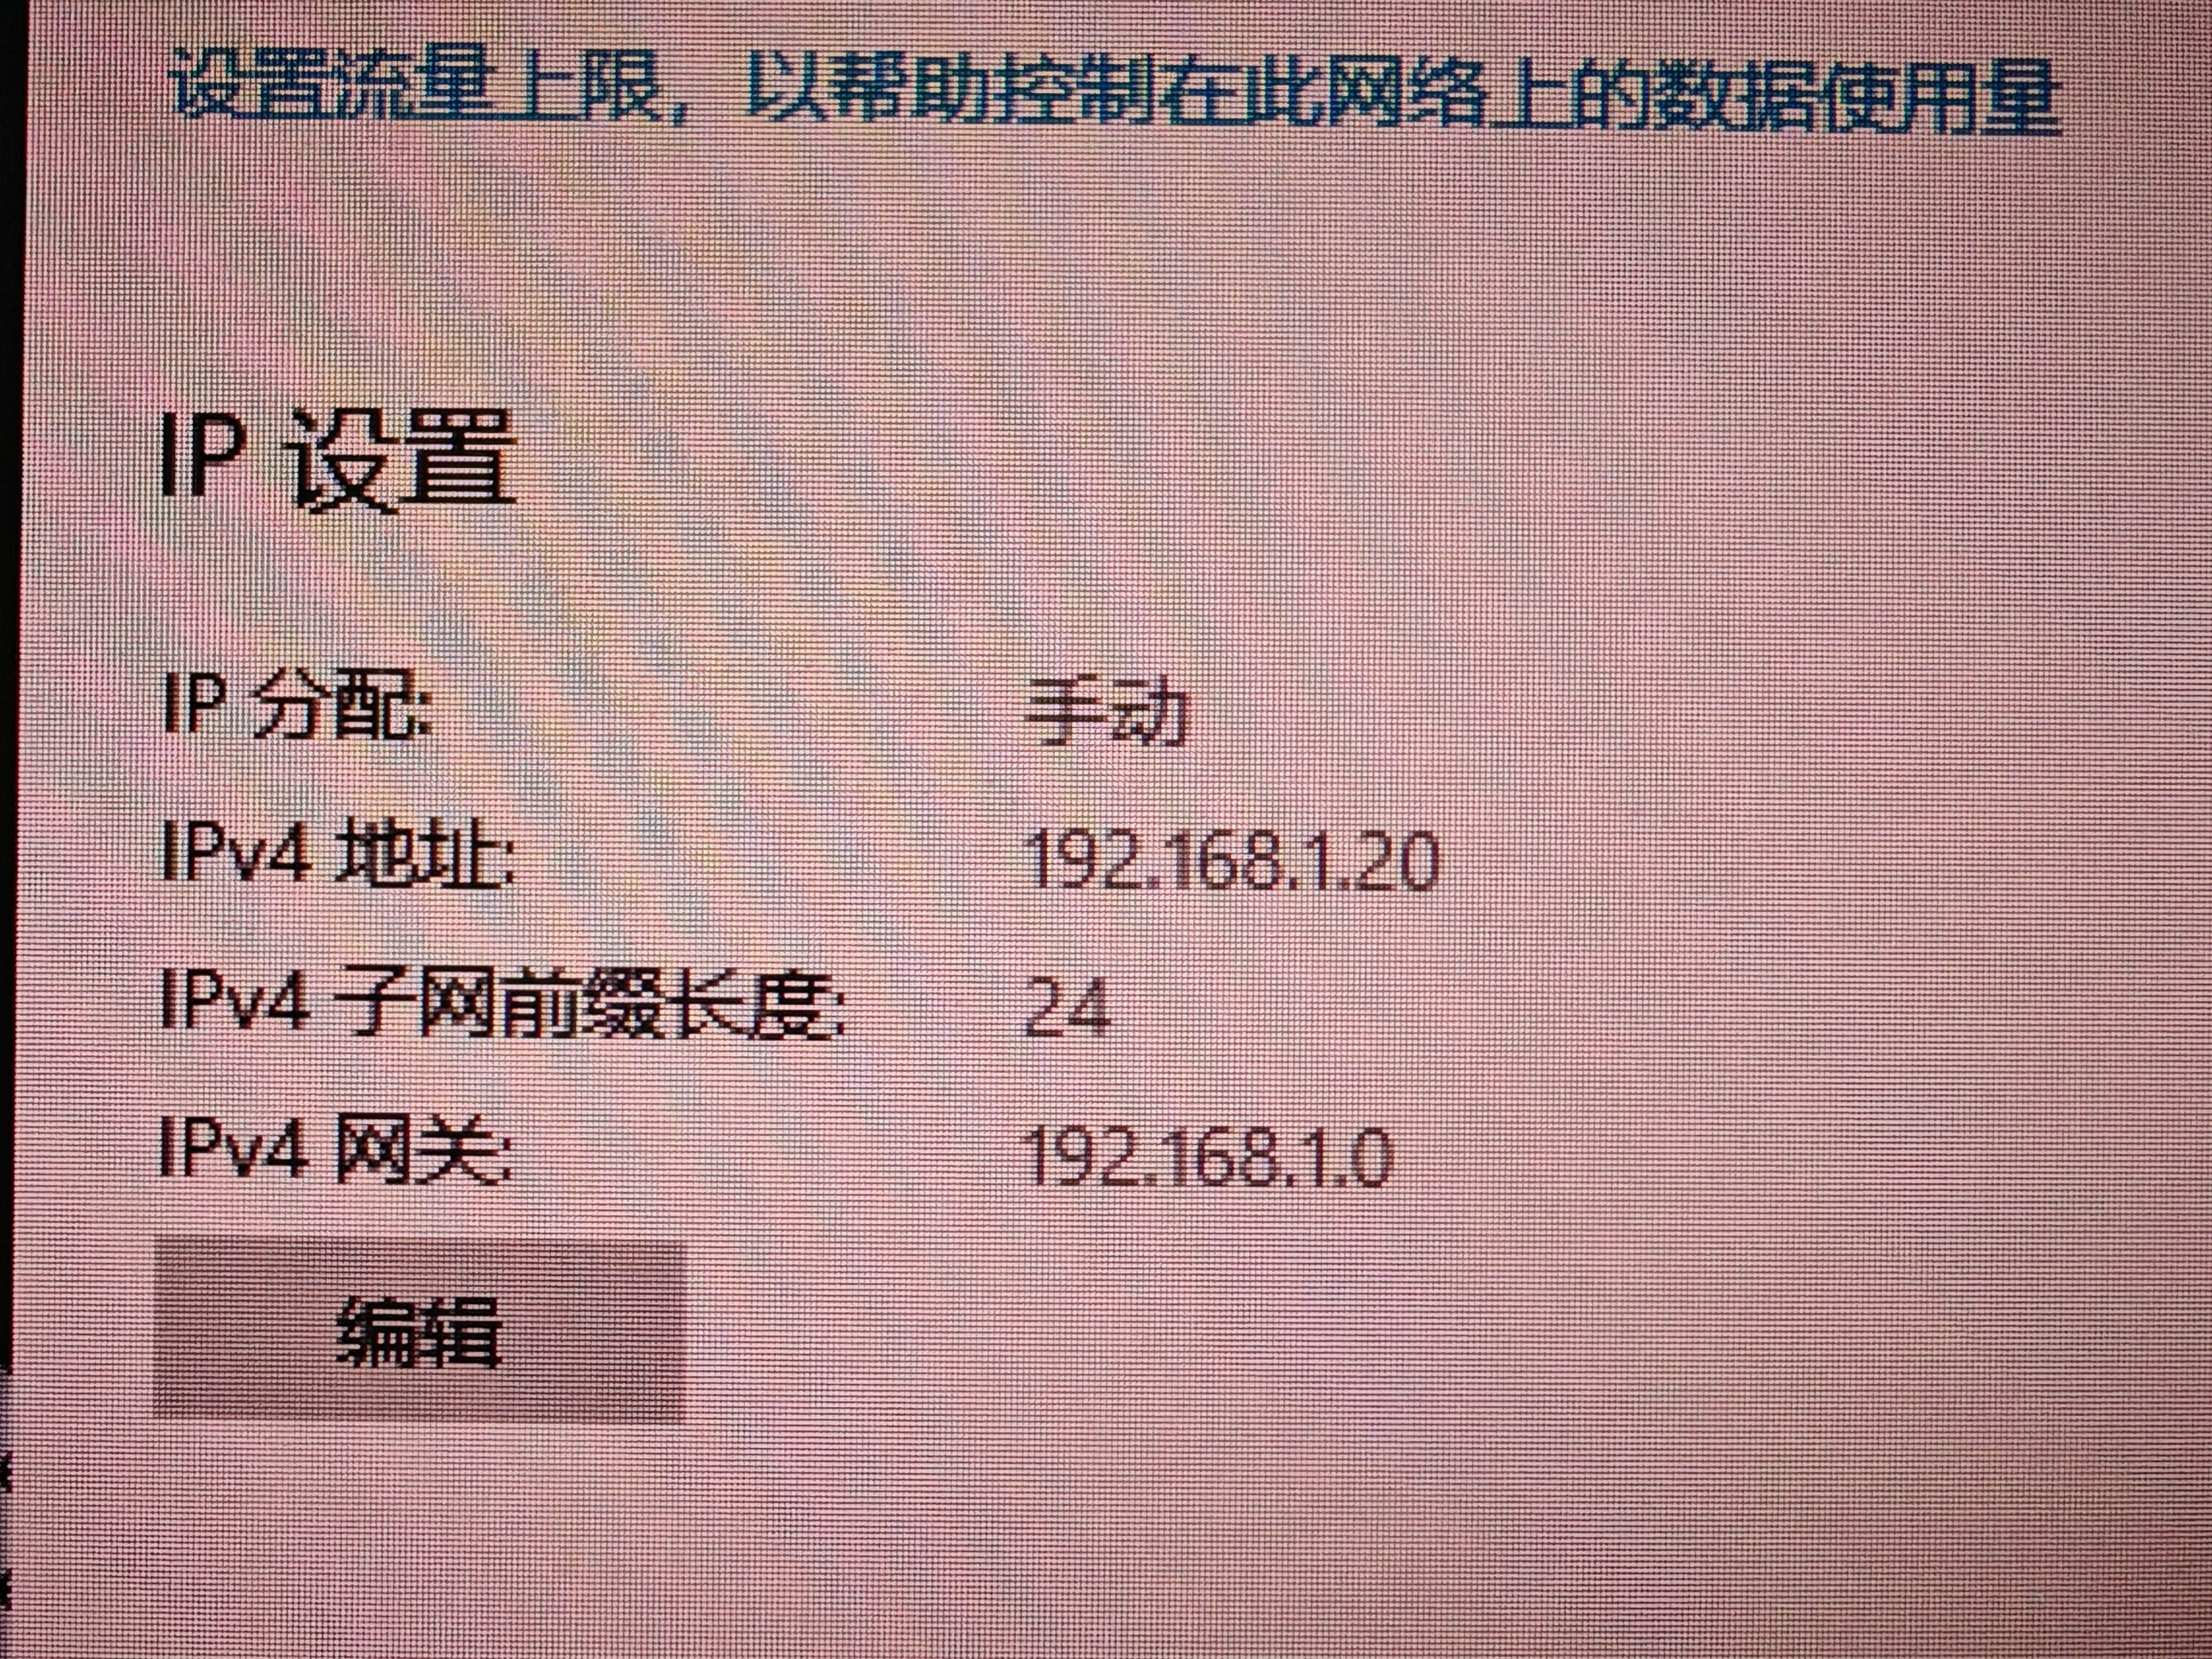
\includegraphics[width=\textwidth]{img/step1/PC2_IP_config.png}
        \caption{PC2的IP地址配置界面}
        \label{fig:PC2_IP_config}
    \end{subfigure}
\end{figure}

\begin{itemize}
    \item PC1配置如上（见图\ref{fig:PC1_IP_config}）：
    \begin{itemize}
        \item IPv4地址：192.168.1.10
        \item 子网前缀长度：24
        \item 网关：192.168.1.0
    \end{itemize}
    \item PC2配置如上（见图\ref{fig:PC2_IP_config}）：
    \begin{itemize}
        \item IPv4地址：192.168.1.20
        \item 子网前缀长度：24
        \item 网关：192.168.1.0
    \end{itemize}
\end{itemize}

\subsubsection{查看并关闭交换机的生成树协议}
为观察环路现象，需先关闭华为交换机默认开启的MSTP。
\begin{itemize}
    \item 交换机A执行\texttt{undo stp enable}，系统提示警告，输入\texttt{y}确认。执行\texttt{display stp}，显示Protocol Status: Disabled（见图\ref{fig:SwitchA_disable_STP}）。
    \item 交换机B同样操作，关闭STP并确认，状态显示为Disabled，桥优先级为默认32768（见图\ref{fig:SwitchB_disable_STP}）。
\end{itemize}

\begin{figure}[H]
    \centering
    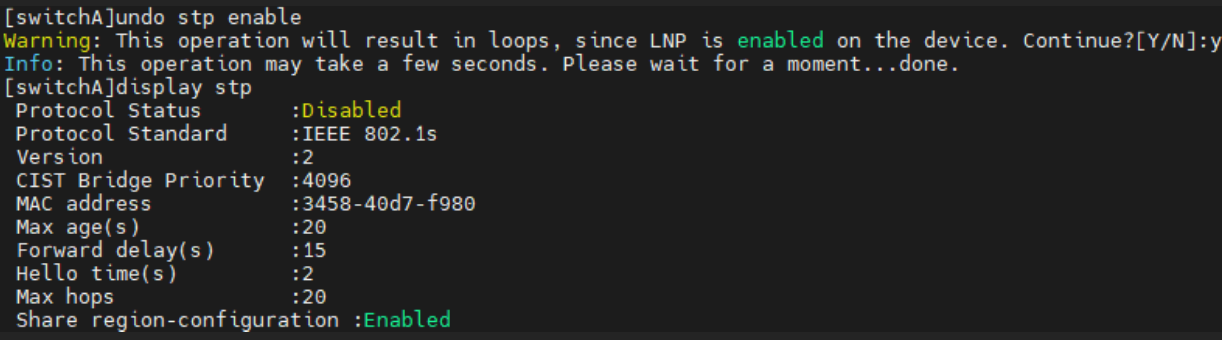
\includegraphics[width=0.7\textwidth]{img/step1/SwitchA_disable_STP.png}
    \caption{SwitchA关闭生成树协议后的状态信息}
    \label{fig:SwitchA_disable_STP}
\end{figure}

\begin{figure}[H]
    \centering
    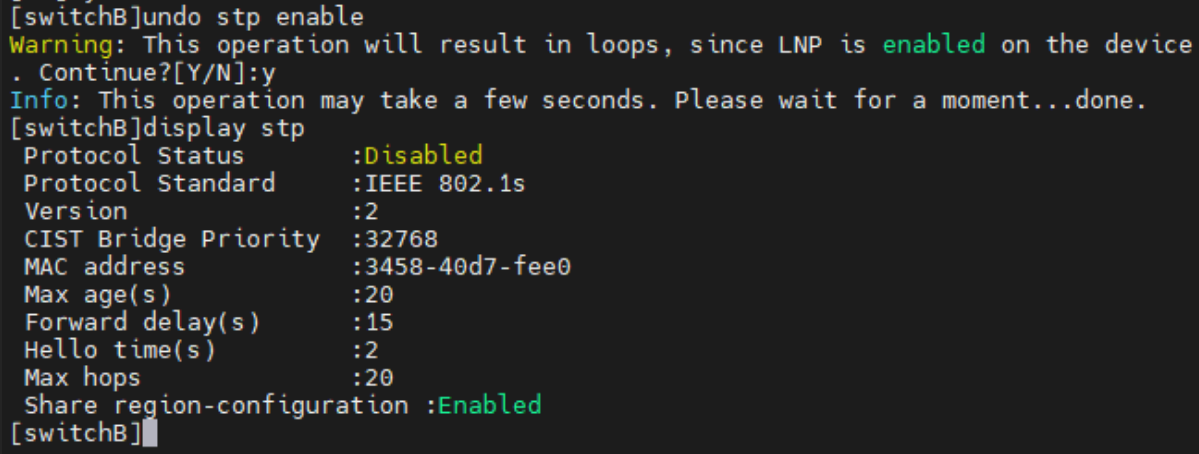
\includegraphics[width=0.7\textwidth]{img/step1/SwitchB_disable_STP.png}
    \caption{SwitchB关闭生成树协议后的状态信息}
    \label{fig:SwitchB_disable_STP}
\end{figure}
操作结果：两台交换机的生成树协议均已关闭，网络失去防环路保护。

\subsubsection{无主动通信状态下环路观察}
\paragraph{实验现象与截图分析}
    \textbf{图1：交换机端口流量利用率}
    \begin{figure}[H]
        \centering
        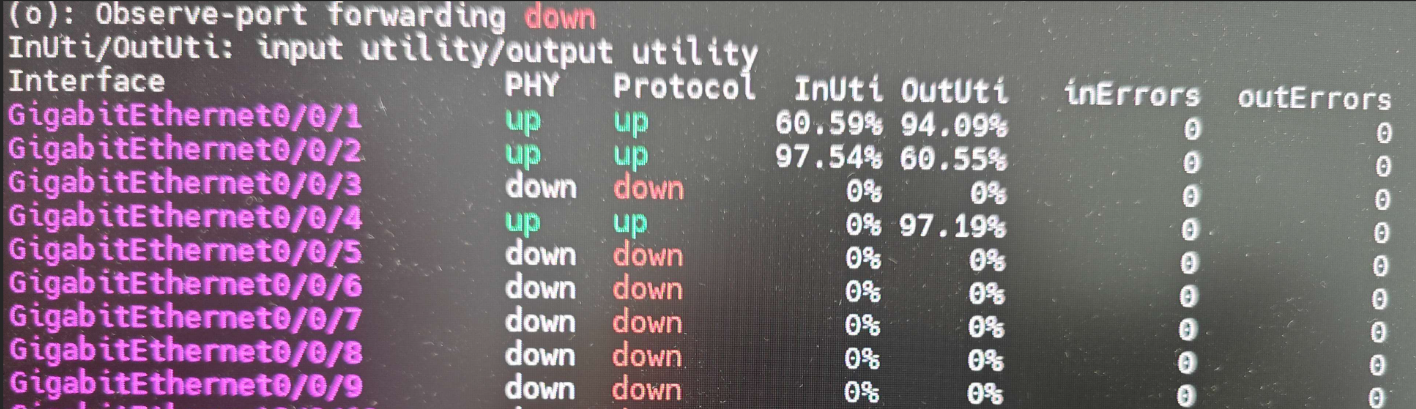
\includegraphics[width=0.7\textwidth]{img/step1/switch_interface_utilization.png}
        \caption{交换机互联端口流量利用率异常（display interface brief）}
    \end{figure}
    \begin{itemize}
        \item \textbf{端口状态：} G0/0/1和G0/0/2均为up，正是两台交换机间的冗余链路，构成物理环路。
        \item \textbf{流量异常：} G0/0/1输入利用率60.59\%，输出94.09\%；G0/0/2输入97.54\%，输出60.55\%。理论上，静默状态下这些端口应接近0\%，如此高的利用率表明链路被大量数据包塞满，是广播风暴的直接证据。
        \item \textbf{其他端口：} 其余端口down且利用率为0\%，说明风暴流量仅在交换机互联端口间循环。
    \end{itemize}
    \textbf{图2：Wireshark抓包内容}
    \begin{figure}[H]
        \centering
        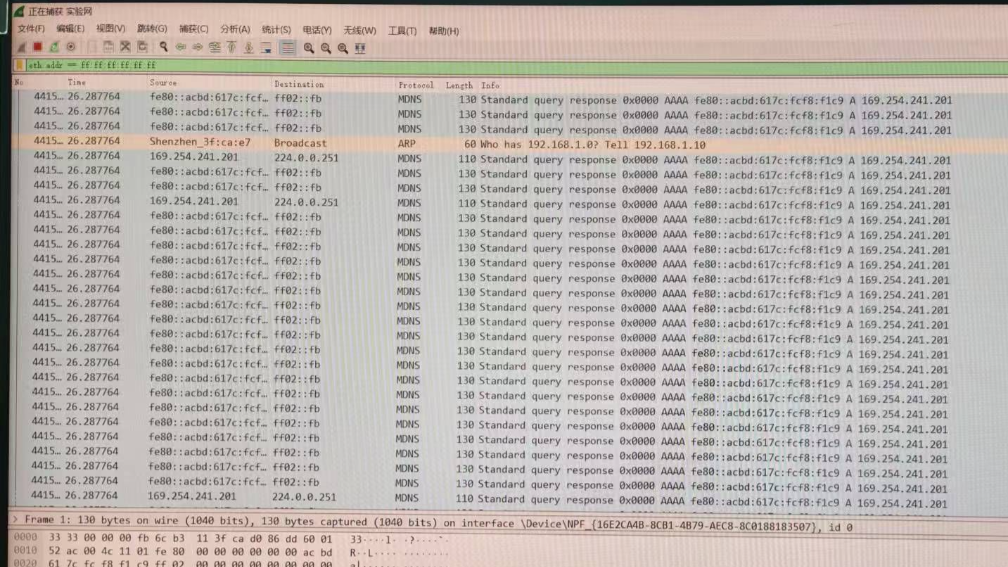
\includegraphics[width=0.7\textwidth]{img/step1/wireshark_broadcast_storm_capture.png}
        \caption{Wireshark抓包显示风暴期间的广播/多播包}
    \end{figure}
    \begin{itemize}
        \item \textbf{时间戳异常：} 多个数据包的Time字段完全相同，说明瞬时包量极大，已超出网卡/驱动计时能力，是广播风暴的典型现象。
        \item \textbf{流量内容：} 既有mDNS（多播DNS）响应包，也有ARP请求（如“Who has 192.168.1.0?”）。这些后台多播/广播流量在环路中被无限复制放大，成为风暴的直接载体。
        \item \textbf{触发源：} 即使无用户主动通信，操作系统后台服务（如Bonjour、ARP探测等）也会周期性发出多播/广播包，足以触发环路中的风暴。
    \end{itemize}

\paragraph{结论}
\begin{itemize}
    \item 只要存在物理环路，即使没有主动通信，后台多播/广播流量也会被无限复制，导致广播风暴。
    \item 交换机互联端口利用率异常升高，抓包显示瞬时大量广播/多播包，是风暴的直接证据。
    \item 生成树协议关闭后，网络缺乏环路保护，极易因后台流量诱发风暴，严重影响网络可用性。
\end{itemize}

\subsubsection{不同Ping操作下数据包增长速率对比}

\textbf{问题回答}

答：第二种情况（ping一个不存在的IP）包增长更快，会迅速触发广播风暴。

下面结合五张图片的具体数据，对两种情况进行详细对比分析。

\textbf{情况一：PC1 ping PC2（正常通信）}

\textbf{流量特征分析}

\begin{itemize}
    \item \textbf{图1：初始流量状态}
    \begin{figure}[H]
        \centering
        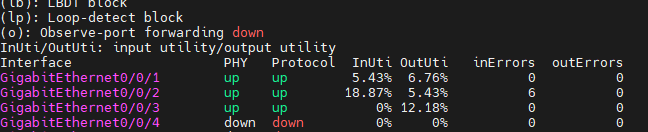
\includegraphics[width=0.7\textwidth]{img/step1/ping_normal_initial.png}
        \caption{正常通信初始流量状态}
    \end{figure}
    \begin{itemize}
        \item G0/0/1输入利用率：5.43\%，G0/0/2输入利用率：18.87\%
        \item 网络初始流量较低，未见异常
    \end{itemize}

    \item \textbf{图2：高负载状态}
    \begin{figure}[H]
        \centering
        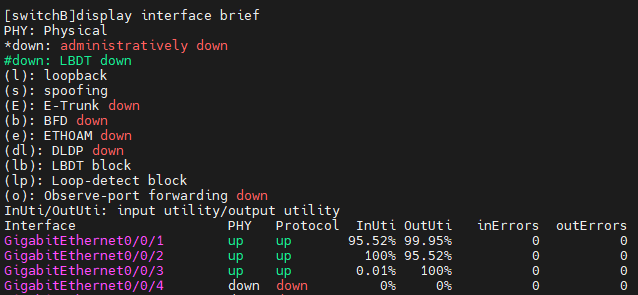
\includegraphics[width=0.7\textwidth]{img/step1/ping_normal_high_load.png}
        \caption{高负载状态}
    \end{figure}
    \begin{itemize}
        \item G0/0/1输入利用率：95.52\%，G0/0/2输入利用率：100\%
    \end{itemize}
\end{itemize}

\textbf{通信机制分析}
\begin{enumerate}
    \item 初始阶段：PC1发送1-2次ARP广播请求解析PC2的MAC地址
    \item 稳定阶段：获得MAC后，通信转为单播ICMP请求/回复
    \item 环路影响：单播包在环路中被有限复制，流量增长相对线性
    \item 最终状态：端口利用率高几乎瘫痪
\end{enumerate}

\textbf{情况二：PC1 ping 不存在IP（触发广播风暴）}

\textbf{流量特征分析}

\begin{itemize}
    \item \textbf{图3：初始安静状态}
    \begin{figure}[H]
        \centering
        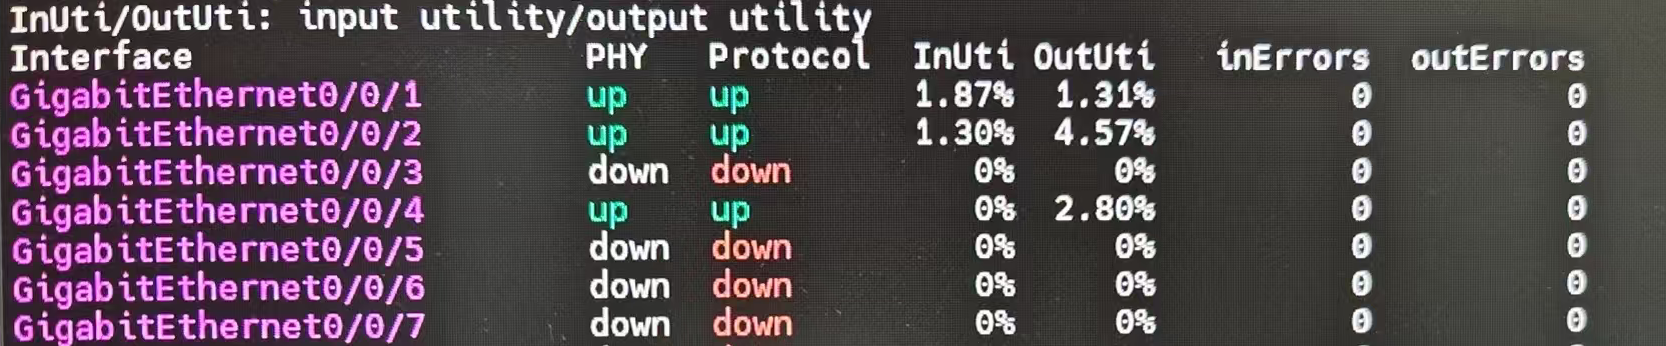
\includegraphics[width=0.7\textwidth]{img/step1/ping_nonexist_initial.png}
        \caption{广播风暴前初始流量状态}
    \end{figure}
    \begin{itemize}
        \item G0/0/1输入利用率：1.87\%，G0/0/2输入利用率：1.30\%
        \item 网络安静，仅有基础流量
    \end{itemize}

    \item \textbf{图4：广播风暴状态}
    \begin{figure}[H]
        \centering
        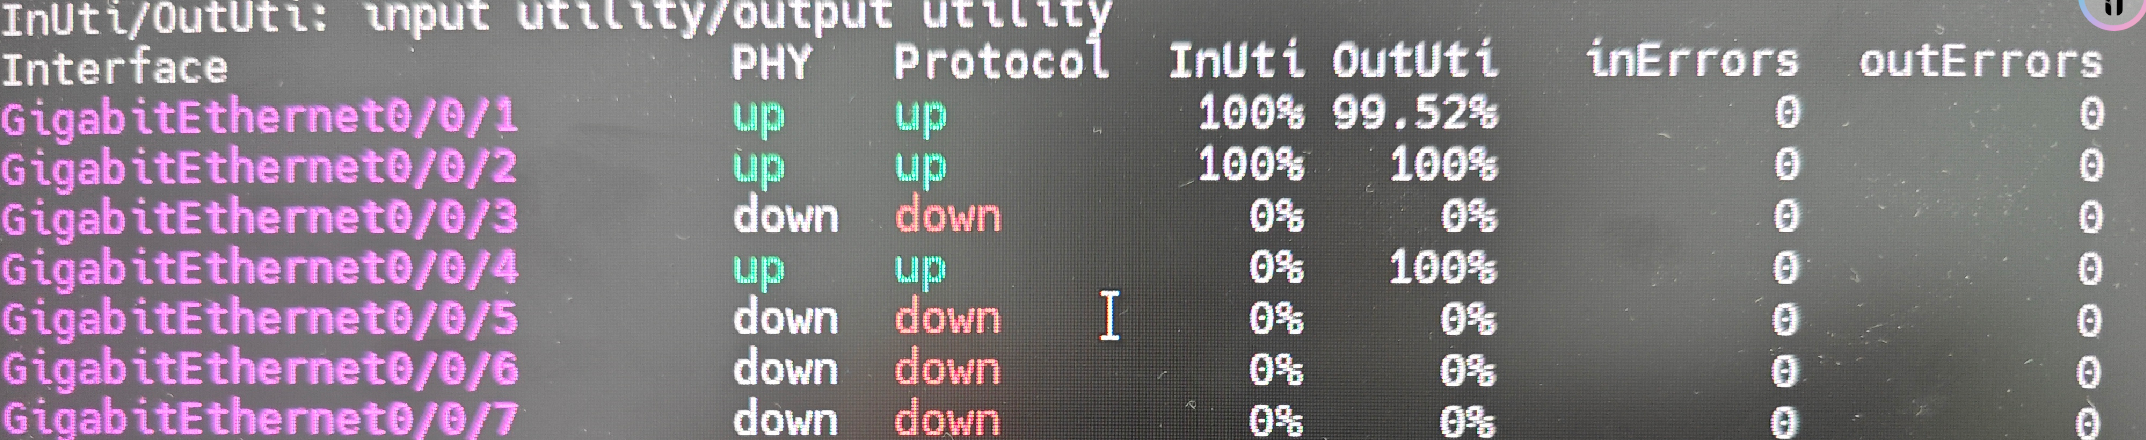
\includegraphics[width=0.7\textwidth]{img/step1/broadcast_storm_full.png}
        \caption{广播风暴时端口利用率100\%}
    \end{figure}
    \begin{itemize}
        \item G0/0/1、G0/0/2输入利用率均为100\%
        \item 网络完全瘫痪
    \end{itemize}
\end{itemize}

\textbf{Wireshark抓包分析}

\begin{figure}[H]
    \centering
    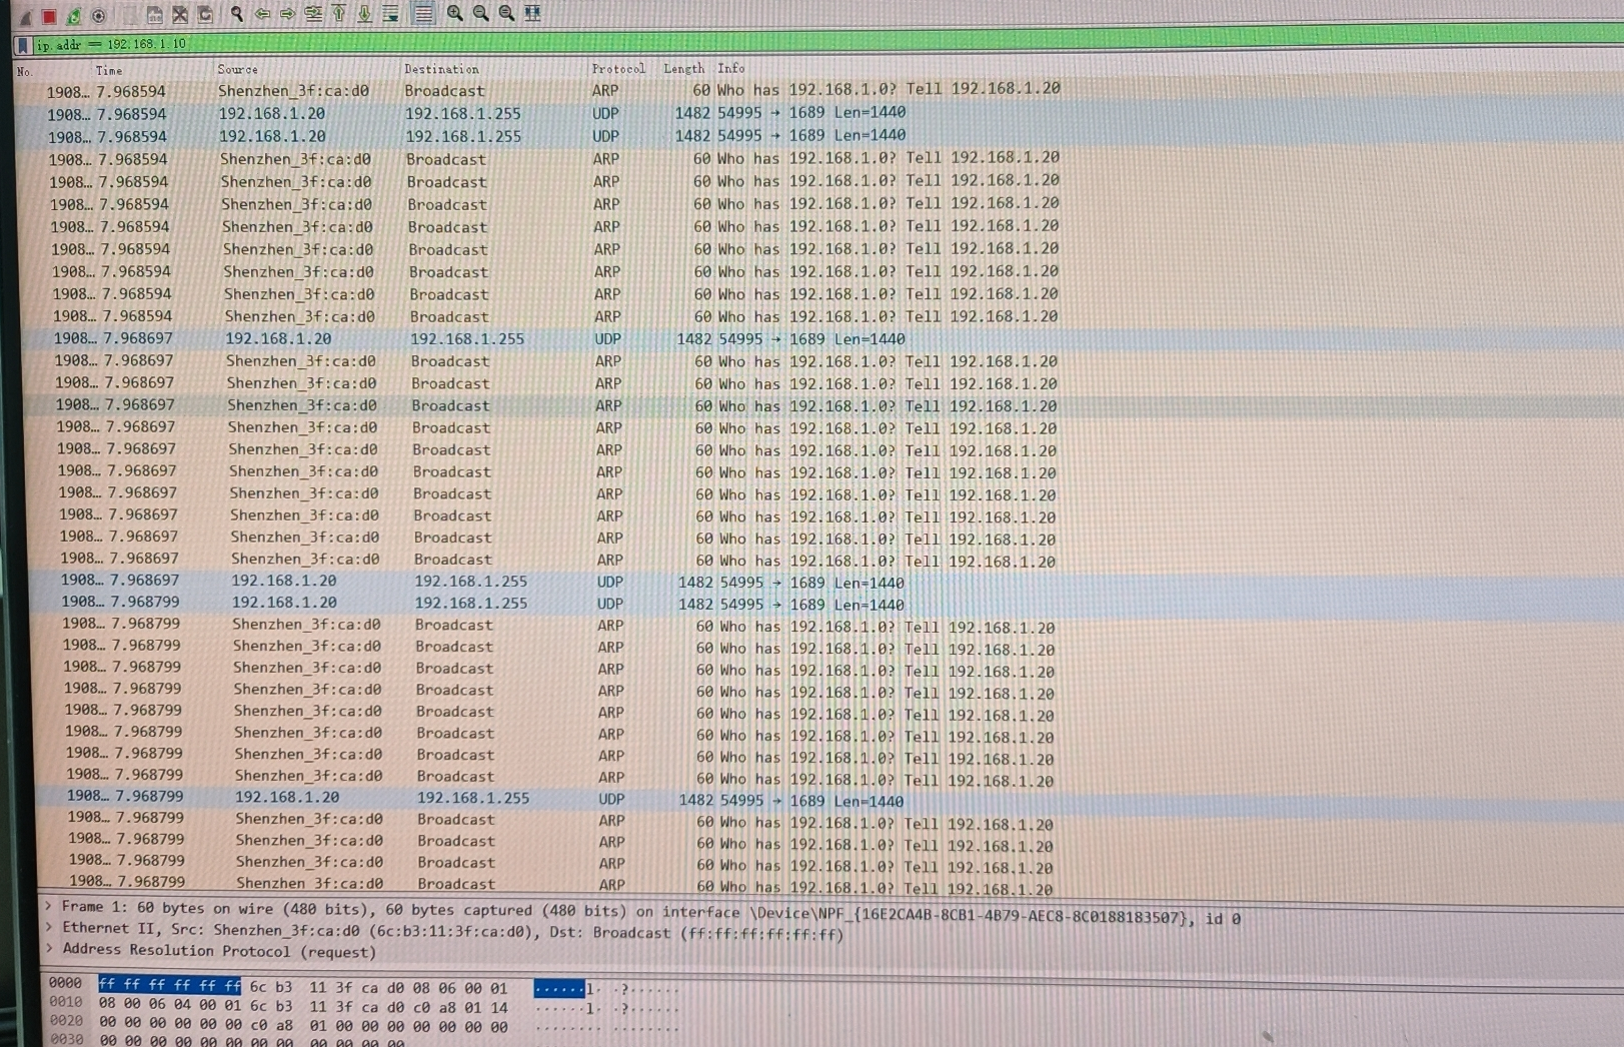
\includegraphics[width=0.7\textwidth]{img/step1/wireshark_storm_capture.png}
    \caption{广播风暴期间Wireshark抓包}
\end{figure}

\begin{itemize}
    \item 海量ARP广播请求："Who has 192.168.1.0? Tell 192.168.1.20"
    \item 多个数据包时间戳完全相同，表明数据包洪泛
    \item 目标地址为192.168.1.255（广播地址）
    \item UDP大包也被卷入风暴
\end{itemize}
\textbf{对比分析与量化结果}

\begin{table}[H]
    \centering
    \begin{tabular}{|p{3cm}|p{4cm}|p{4cm}|p{3cm}|}
        \hline
        对比指标 & 情况一（ping PC2） & 情况二（ping不存在IP） & 差异分析 \\
        \hline
        触发流量类型 & 单播ICMP为主 & 广播ARP为主 & 广播帧更易被泛洪 \\
        \hline
        环路放大效应 & 线性增长 & 指数级增长 & 情况二放大效应更强 \\
        \hline
        达到饱和时间 & 相对较慢 & 极快（数秒内） & 情况二更快达到100\% \\
        \hline
        端口利用率 & G0/0/1: 95.52\% \newline G0/0/2: 100\% & G0/0/1: 100\% \newline G0/0/2: 100\% & 情况二完全饱和 \\
        \hline
        网络恢复能力 & 仍可勉强通信 & 完全瘫痪 & 情况二影响更严重 \\
        \hline
    \end{tabular}
    \caption{两种Ping操作下流量增长速率对比}
\end{table}


\subsubsection{观察交换机MAC地址表的变化}

广播风暴时，分别在两个时刻查看SwitchB的MAC地址表。

\begin{itemize}
    \item 时刻1：显示四条动态学习的MAC地址，分别从GE0/0/1和GE0/0/2端口学习（见图\ref{fig:MAC_table_moment1}）。
    \item 时刻2：同样四条MAC地址，但全部显示从GE0/0/2端口学习，部分MAC的学习端口发生变化（见图\ref{fig:MAC_table_moment2}）。
\end{itemize}

\begin{figure}[H]
    \centering
    \begin{subfigure}[b]{0.45\textwidth}
        \centering
        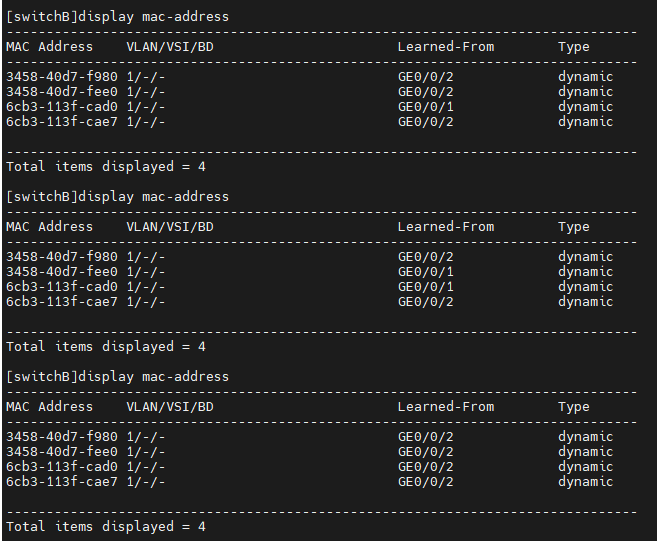
\includegraphics[width=\textwidth]{img/step1/MAC_table_moment1.png}
        \caption{广播风暴中某一时刻SwitchB的MAC地址表}
        \label{fig:MAC_table_moment1}
    \end{subfigure}
    \hfill
    \begin{subfigure}[b]{0.45\textwidth}
        \centering
        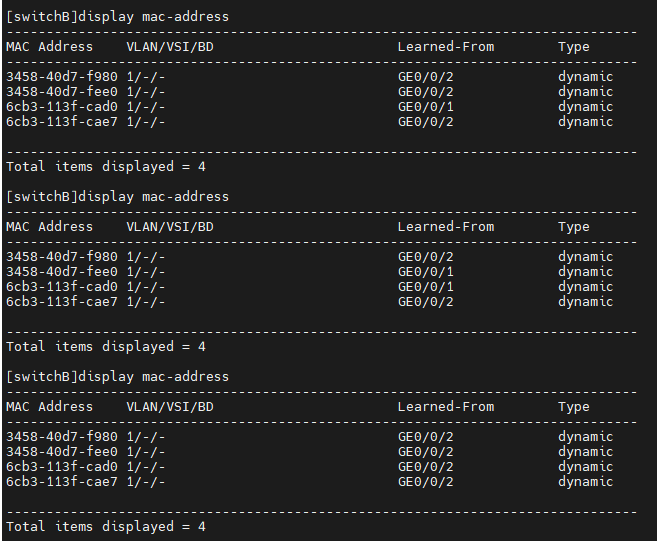
\includegraphics[width=\textwidth]{img/step1/MAC_table_moment2.png}
        \caption{几秒后，同一交换机MAC地址表显著变化}
        \label{fig:MAC_table_moment2}
    \end{subfigure}
\end{figure}

实验结论：广播风暴导致MAC地址表震荡，交换机频繁、错误地更新MAC与端口的映射，影响转发性能。

\subsubsection{步骤一小结}

\begin{itemize}
    \item \textbf{广播风暴的产生条件：} 需同时具备物理环路和广播帧（如ARP请求）。
    \item \textbf{ping不存在IP为何流量更大：} 因持续ARP请求得不到响应，广播帧被无限复制，流量爆炸式增长。
    \item \textbf{MAC地址表震荡危害：} 导致转发错误、CPU负担加重、转发效率下降，甚至泛洪。
\end{itemize}

\subsection{步骤二和三：交换机基本配置}
\subsubsection{步骤二：交换机A基本配置}

\begin{lstlisting}[language=bash]
<S5720-02-1>system-view
[SwitchA]sysname switchA
[switchA]vlan 10
[switchA-vlan10]name sales
[switchA]interface GigabitEthernet0/0/3
[switchA-GigabitEthernet0/0/3]port link-type access
[switchA-GigabitEthernet0/0/3]port default vlan 10
[switchA]port-group pg1
[switchA-port-group-pg1]group-member GigabitEthernet0/0/1 to GigabitEthernet0/0/2
[switchA-port-group-pg1]port link-type trunk
[switchA-port-group-pg1]port trunk allow-pass vlan 10
\end{lstlisting}

\subsubsection{步骤三：交换机B基本配置}

\begin{lstlisting}[language=bash]
<S5720-02-2>system-view
[SwitchB]sysname switchB
[switchB]vlan 10
[switchB-vlan10]name sales
[switchB]interface GigabitEthernet0/0/3
[switchB-GigabitEthernet0/0/3]port link-type access
[switchB-GigabitEthernet0/0/3]port default vlan 10
[switchB]port-group pg1
[switchB-port-group-pg1]group-member GigabitEthernet0/0/1 to GigabitEthernet0/0/2
[switchB-port-group-pg1]port link-type trunk
[switchB-port-group-pg1]port trunk allow-pass vlan 10
\end{lstlisting}
配置结果如下图所示：
\begin{figure}[H]
    \centering
    \begin{subfigure}[b]{0.45\textwidth}
        \centering
        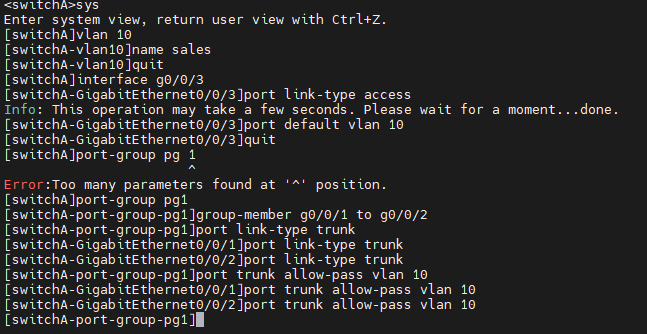
\includegraphics[width=\textwidth]{img/step2to3/switchA_basic_config.png}
        \caption{交换机A的基本配置结果}
        \label{fig:SwitchA_basic_configuration}
    \end{subfigure}
    \hfill
    \begin{subfigure}[b]{0.45\textwidth}
        \centering
        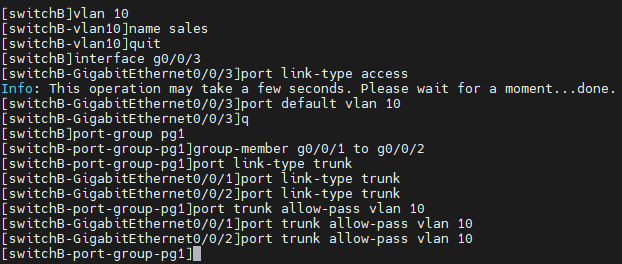
\includegraphics[width=\textwidth]{img/step2to3/switchB_basic_config.png}
        \caption{交换机B的基本配置结果}
        \label{fig:SwitchB_basic_configuration}
    \end{subfigure}
\end{figure}

\subsection{步骤四：配置RSTP}

\subsubsection{配置交换机A的RSTP}

在交换机A上执行快速生成树协议的配置命令:
\begin{lstlisting}[language=bash]
[switchA]stp enable
Warning: The global STP state will be changed. Continue?[Y/N]:y
Info: This operation may take a few seconds. Please wait for a moment...done.
[switchA]stp mode rstp
\end{lstlisting}

\begin{figure}[H]
    \centering
    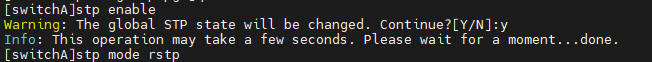
\includegraphics[width=0.7\textwidth]{img/step4/switchA_RSTP_configuration.png}
    \caption{交换机A的RSTP配置过程}
\end{figure}

\subsubsection{配置交换机B的RSTP}
在交换机B上执行与交换机A相同的RSTP配置命令。
\begin{lstlisting}[language=bash]
[switchB]stp enable
Warning: The global STP state will be changed. Continue?[Y/N]:y
Info: This operation may take a few seconds. Please wait for a moment...done.
[switchB]stp mode rstp
\end{lstlisting}
\begin{figure}[H]
    \centering
    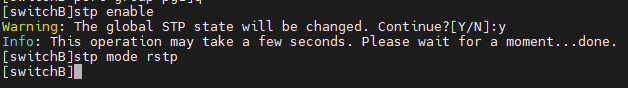
\includegraphics[width=0.7\textwidth]{img/step4/switchB_STP_mode_to_RSTP.png}
    \caption{交换机B的RSTP配置过程}
\end{figure}
首先执行stp enable命令全局启用生成树协议，系统提示警告信息，确认后操作完成。接着执行stp mode rstp命令将生成树协议模式设置为快速生成树协议。系统提示操作需要几秒钟时间，最终完成RSTP配置。

\subsubsection{验证RSTP配置状态}
配置完成后，通过display stp命令验证两台交换机的RSTP运行状态。
\begin{lstlisting}[language=bash]
[switchA]display stp
\end{lstlisting}

\begin{figure}[H]
    \centering
    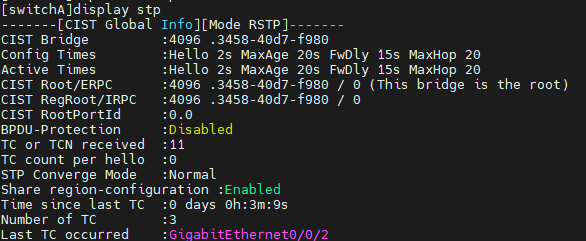
\includegraphics[width=0.7\textwidth]{img/step4/switchA_spanning_tree_status.png}
    \caption{交换机A的RSTP全局状态信息}
\end{figure}
关键信息包括：运行模式为RSTP，桥ID为4096.3458-40d7-f980（优先级4096，MAC地址3458-40d7-f980），本交换机为根桥，根路径开销为0，协议定时器为Hello Time 2s、MaxAge 20s、Forward Delay 15s，拓扑变更统计显示接收到11次TC报文，发生了3次拓扑变更。

\subsubsection{网络连通性测试}
启用RSTP后，重新用两根跳线将两台交换机按照拓扑图连接起来，形成物理环路，然后重复步骤一的测试。 首先在PC1上持续ping PC2，观察通信是否稳定。
\begin{lstlisting}[language=bash]
C:\Users\Administrator>ping 192.168.1.20 -t
\end{lstlisting}

\begin{figure}[H]
    \centering
    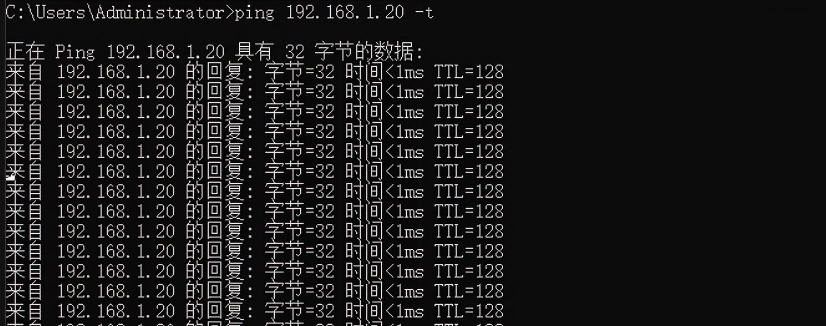
\includegraphics[width=0.7\textwidth]{img/step4/ping_test_result.png}
    \caption{PC1持续ping PC2的测试结果}
\end{figure}
表明在启用RSTP后，即使存在物理环路，网络连通性依然正常。这是因为RSTP通过阻塞冗余端口，打破了环路，确保数据沿生成树的最优路径转发。

\subsubsection{MAC地址表稳定性验证：配置RSTP后的效果}

\begin{figure}[H]
    \centering
    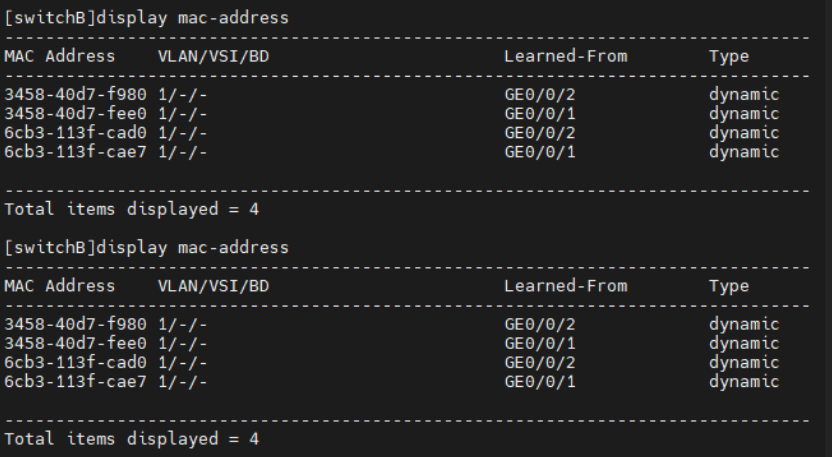
\includegraphics[width=0.7\textwidth]{img/step4/MAC_table_moment.png}
    \caption{RSTP生效后SwitchB连续两次查询MAC地址表，内容完全一致}
    \label{fig:MAC_table_moment}
\end{figure}

\paragraph{图片解析}
此截图展示了在交换机B上连续执行两次 \texttt{display mac-address} 命令的输出结果，是验证快速生成树协议（RSTP）生效后网络层状态稳定的关键证据。

\paragraph{关键信息解读}
\begin{enumerate}
    \item \textbf{MAC地址表内容完全一致} \\
    第一行输出：\texttt{[switchB]display mac-address} 后的MAC地址表。\\
    第二行输出：间隔一段时间后，再次执行相同命令的结果。\\
    核心发现：两次显示的4条动态学习到的MAC地址条目完全一样，包括MAC地址、学习端口、VLAN ID等信息均无任何差异，表明MAC地址表在这段时间内未发生任何变化。
    \item \textbf{具体条目分析}
    \begin{table}[H]
        \centering
        \begin{tabular}{|c|c|c|c|}
            \hline
            MAC地址 & 学习端口 & 设备推测 & 状态分析 \\
            \hline
            3458-40d7-f980 & GE0/0/2 & 可能是交换机A或其它设备 & 端口固定，无变化 \\
            3458-40d7-fee0 & GE0/0/1 & 可能是交换机A或其它设备 & 端口固定，无变化 \\
            6cb3-113f-cad0 & GE0/0/2 & 可能是终端设备 & 端口固定，无变化 \\
            6cb3-113f-cae7 & GE0/0/1 & 可能是终端设备 & 端口固定，无变化 \\
            \hline
        \end{tabular}
        \caption{MAC地址表条目分析}
    \end{table}
    关键观察：每个MAC地址都有确定且唯一的端口映射，且在两次查询中保持绝对不变。
\end{enumerate}

\paragraph{与步骤一实验的对比分析}
\begin{itemize}
    \item \textbf{步骤一（未启用RSTP）状态回顾} \\
    在存在物理环路且未启用生成树协议时，MAC地址出现剧烈震荡：
    \begin{itemize}
        \item 同一MAC地址在不同时刻从不同端口学习
        \item 表示MAC地址与端口映射关系频繁错误更新
        \item 这是广播风暴和二层环路的直接证据
    \end{itemize}
    \item \textbf{当前状态（启用RSTP后）分析} \\
    当前截图证明RSTP已成功解决上述问题：
    \begin{itemize}
        \item \textbf{环路消除机制生效}：RSTP通过选举阻塞了冗余端口（如SwitchB的G0/0/2），数据帧在逻辑无环的拓扑中传输，交换机不再从多个端口收到同一设备的数据帧。
        \item \textbf{MAC学习机制稳定}：每个设备的数据帧沿确定路径到达交换机，交换机能够正确、稳定地学习MAC地址与端口映射，学习到的条目在地址表中持久保持。
        \item \textbf{网络收敛状态}：两次查询结果完全一致，表明网络处于稳定收敛状态，无拓扑变化，无MAC地址表更新，这是网络健康运行的标志。
    \end{itemize}
\end{itemize}


\subsubsection{广播风暴验证}
为了验证RSTP对广播风暴的防护效果，进行网络数据包捕获分析。 使用Wireshark在PC1上抓包，观察网络流量情况。
\begin{figure}[H]
    \centering
    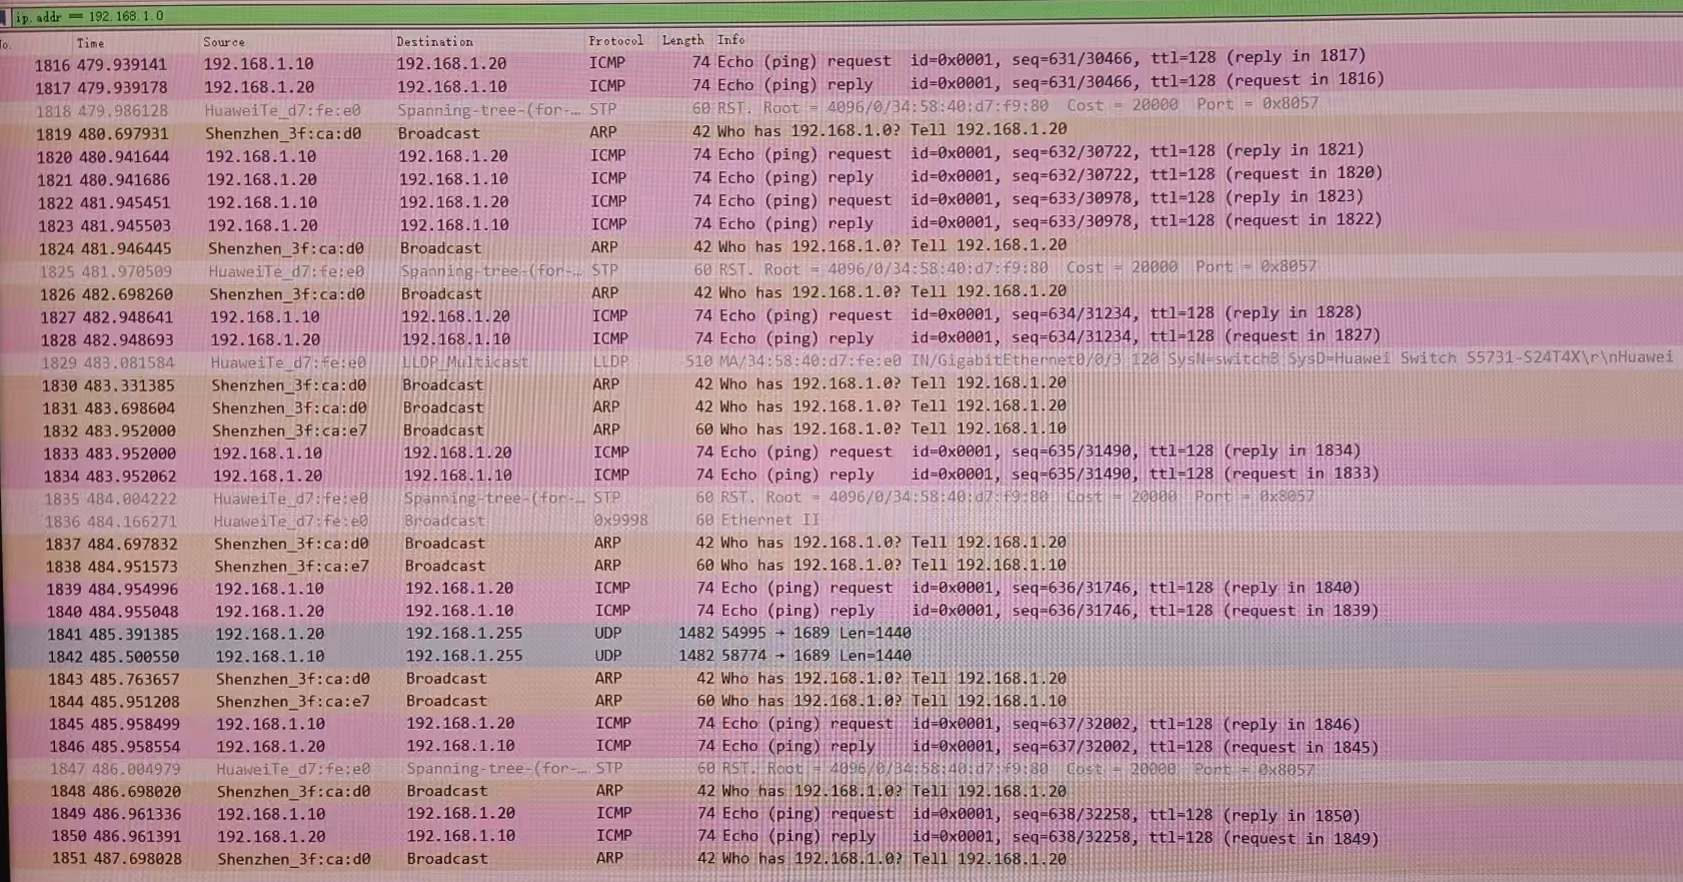
\includegraphics[width=0.7\textwidth]{img/step4/network_packet_capture.png}
    \caption{Wireshark网络数据包捕获截图}
\end{figure}
捕获的数据包显示了正常的网络通信，包括ICMP协议（PC1与PC2之间的ping通信）、ARP协议（必要的地址解析协议通信）、STP协议（生成树协议的BPDU报文）。无海量ARP广播请求，无数据包循环复制现象。与步骤一未启用RSTP时的广播风暴对比，启用RSTP后网络流量正常，无广播风暴迹象。

\subsubsection{配置前后实验效果对比}

通过重复步骤一的测试，对比启用RSTP前后的实验效果：
\begin{table}[H]
    \centering
    \small
    \setlength{\tabcolsep}{2pt}
    \begin{tabular}{|p{2.5cm}|p{3.5cm}|p{3.5cm}|p{4cm}|}
        \hline
        测试项目 & 启用RSTP前 & 启用RSTP后 & 分析 \\
        \hline
        广播风暴 & 存在，ping不存在IP时触发 & 不存在 & RSTP阻塞冗余端口，打破逻辑环路 \\
        \hline
        MAC地址表 & 震荡，不稳定 & 稳定 & 无环路，MAC地址学习正常 \\
        \hline
        网络连通性 & 可能不通或丢包严重 & 稳定连通，无丢包 & 数据沿生成树确定的最优路径转发 \\
        \hline
        端口状态 & 所有活动端口转发 & 部分端口阻塞 & RSTP选举端口角色，阻塞冗余链路 \\
        \hline
        网络负载 & 高，接近100\% & 正常 & 无广播帧无限循环 \\
        \hline
    \end{tabular}
    \caption{启用RSTP前后实验效果对比}
\end{table}
\subsubsection{步骤四小结}
通过本实验，验证了生成树协议（特别是RSTP）在网络中的关键作用：
\begin{itemize}
    \item \textbf{环路消除：} 逻辑阻塞交换机B的G0/0/1端口（Disable状态），打破物理环路，防止广播风暴。
    \item \textbf{根桥选举：} 根据桥优先级（数值越小优先级越高），交换机A（优先级4096）被选举为根桥，交换机B（默认优先级32768）为非根桥。
    \item \textbf{路径优化：} 交换机B的G0/0/2端口被选举为根端口（到根桥的最优路径），处于转发状态，负责数据传输。
    \item \textbf{冗余备份：} 当活动的根端口故障时，被阻塞的备用端口可以快速转换为转发状态，提供网络冗余。
    \item \textbf{网络稳定：} 确保MAC地址表稳定，防止多帧复制和MAC地址表震荡。
\end{itemize}

\subsection{步骤五至八：端口状态与根桥优先级验证}

\subsubsection{步骤五（一）：端口状态验证}

RSTP配置完成后5秒，在交换机B上使用 \texttt{display stp interface} 命令查看互联端口状态：

\begin{lstlisting}[language=bash]
[switchB]display stp interface GigabitEthernet0/0/1
----[Port85(GigabitEthernet0/0/1)][DOWN]----
Port Role :Disabled Port
Port Cost(Dot1T) :Config=auto / Active=20000000
Designated Bridge/Port :32768.3458-40d7-fee0 / 128.85
BPDU Sent :0
BPDU Received :0
\end{lstlisting}

\begin{figure}[H]
    \centering
    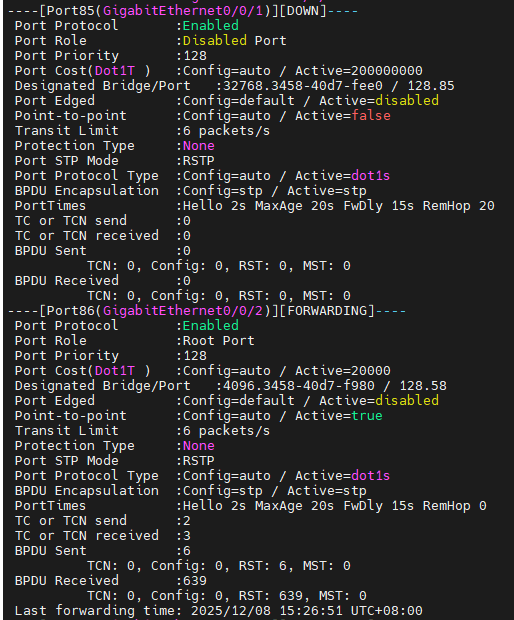
\includegraphics[width=0.6\textwidth]{img/step5to8/switchB_g0_0_1_stp_status.png}
    \caption{交换机B端口G0/0/1的STP状态}
    \label{fig:switchB_g0_0_1_stp_status}
\end{figure}

\begin{lstlisting}[language=bash]
[switchB]display stp interface GigabitEthernet0/0/2
----[Port86(GigabitEthernet0/0/2)][FORWARDING]----
Port Role :Root Port
Port Cost(Dot1T) :Config=auto / Active=20000
Designated Bridge/Port :4096.3458-40d7-f980 / 128.58
Last forwarding time: 2025/12/08 15:26:51 UTC+08:00
\end{lstlisting}

分析：G0/0/1为Disabled Port（丢弃），G0/0/2为Root Port（转发），RSTP已阻塞冗余端口，消除环路。

\subsubsection{步骤五（二） 根交换机与根端口判断}

通过 \texttt{display stp} 命令查看全局信息：

\begin{lstlisting}[language=bash]
[switchA]display stp
-------[CIST Global Info][Mode RSTP]-------
CIST Bridge         :4096.3458-40d7-f980
CIST Root/ERPC      :4096.3458-40d7-f980/0(This bridge is the root)
CIST RootPortId     :0.0
Number of TC        :3
\end{lstlisting}

\begin{figure}[H]
    \centering
    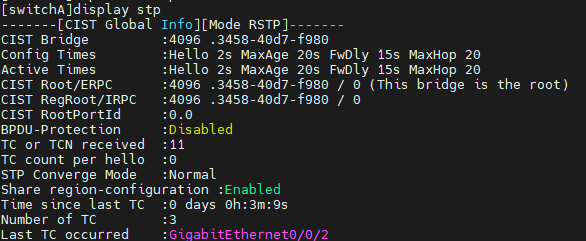
\includegraphics[width=0.7\textwidth]{img/step5to8/switchA_stp_global_info.png}
    \caption{交换机A的STP全局信息}
    \label{fig:switchA_stp_global_info}
\end{figure}

\begin{lstlisting}[language=bash]
[switchB]display stp
-------[CIST Global Info][Mode RSTP]-------
CIST Bridge         :32768.3458-40d7-fee0
CIST Root/ERPC      :4096.3458-40d7-f980 / 20000
CIST RootPortId     :128.85 (GigabitEthernet0/0/1)
\end{lstlisting}

判断：交换机A为根桥（优先级4096），交换机B的根端口为G0/0/1。根桥选举依据桥ID，优先级数值越小优先级越高。

\subsubsection{步骤六：设置交换机优先级}

为确保交换机A被选为根桥，设置其优先级：

\begin{lstlisting}[language=bash]
[switchA]stp priority 4096
\end{lstlisting}

\subsubsection{步骤七：验证优先级配置}

配置完成后，验证交换机A优先级：

\begin{lstlisting}[language=bash]
[switchA]display stp
CIST Bridge :4096.3458-40d7-f980
CIST Root/ERPC :4096.3458-40d7-f980/0(This bridge is the root)
\end{lstlisting}
可以查看上图\ref{fig:switchA_stp_global_info}中显示的桥ID，优先级已变为4096。

对比分析：启用RSTP后，优先级配置生效，网络由无防环路保护转变为受控树形拓扑。高优先级（数值小）端口转发，低优先级端口丢弃；优先级相同则通过端口号较小者转发。

\subsubsection{步骤八：详细验证端口状态}
交换机B端口详细状态：
\begin{lstlisting}[language=bash]
[switchB]display stp interface GigabitEthernet0/0/1
----[Port85(GigabitEthernet0/0/1)][FORWARDING]----
Port Protocol       :Enabled
Port Role           :Root Port
Port Priority       :128
Port Cost(Dot1T )   :Config=auto / Active=20000
Designated Bridge/Port   :4096.3458-40d7-f980 / 128.57
BPDU Sent           :43
BPDU Received       :272
Last forwarding time: 2025/12/08 15:13:16 UTC+08:00
\end{lstlisting}

\begin{lstlisting}[language=bash]
[switchB]display stp interface GigabitEthernet0/0/2
----[Port86(GigabitEthernet0/0/2)][DISCARDING]----
Port Protocol       :Enabled
Port Role           :Alternate Port
Port Priority       :128
Port Cost(Dot1T )   :Config=auto / Active=20000
Designated Bridge/Port   :4096.3458-40d7-f980 / 128.57
BPDU Sent           :2
BPDU Received       :128
\end{lstlisting}

问题解答：
\begin{itemize}
    \item 交换机B的端口0/0/1处于什么状态？\textbf{FORWARDING}
    \item 交换机B的端口0/0/1的端口角色是什么？\textbf{Root Port}
    \item 交换机B的端口0/0/2处于什么状态？\textbf{DISCARDING}
    \item 交换机B的端口0/0/2的端口角色是什么？\textbf{Alternate Port}
\end{itemize}

端口角色与状态对应关系如下：

\begin{table}[H]
    \centering
    \begin{tabular}{|c|c|c|c|}
        \hline
        端口 & 角色 & 状态 & 作用 \\
        \hline
        G0/0/1 & Root Port & FORWARDING & 到根桥的最佳路径，转发所有数据 \\
        G0/0/2 & Alternate Port & DISCARDING & 备用路径，监视网络状态但不转发数据 \\
        G0/0/3 & Designated Port & FORWARDING & 接入PC，转发数据 \\
        \hline
    \end{tabular}
    \caption{端口角色与状态对应关系}
\end{table}
端口统计分析：G0/0/1发送43、接收272个BPDU，G0/0/2发送2、接收128个BPDU。根端口活跃交换BPDU，备用端口主要接收BPDU进行监控。两个端口开销均为20000（千兆以太网默认），开销相同则通过端口优先级决定根端口。

\subsubsection{实验五至八小结}

通过步骤五至八的实验，验证了RSTP核心原理：
\begin{itemize}
    \item \textbf{根桥选举机制：} 桥ID由优先级和MAC地址组成，优先级数值越小优先级越高，优先级相同时比较MAC地址。
    \item \textbf{端口角色分配：} 根端口（最佳路径，转发），指定端口（网段转发），备用端口（冗余备份，丢弃）。
    \item \textbf{环路防止策略：} 阻塞冗余端口，形成无环树形拓扑，故障时备用端口可快速转发。
    \item \textbf{RSTP快速收敛特性：} 端口状态快速切换，秒级收敛，提升网络可靠性。
\end{itemize}

\subsection{步骤九：实验分析}
\subsubsection{正常状态下生成树信息记录}
经过优先级设置后，记录两台交换机的生成树信息如下：
\begin{table}[H]
    \centering
    \begin{tabular}{|c|c|c|c|}
        \hline
        属性 & 描述 & 交换机A & 交换机B \\
        \hline
        Port Priority & 网桥优先权 & 32768 & 32768 \\
        CIST Bridge & 本机网桥ID & 32768.3458-40d7-fe00 & 32768.3458-40d7-fee0 \\
        CIST Root/ERPC & 根桥ID/外部路径开销 & 4096.3458-40d7-f980 / 20000 & 4096.3458-40d7-f980 / 20000 \\
        CIST RootPortId & 根端口 & - & 128.86 (GigabitEthernet0/0/2) \\
        Designated & 指定端口 & - & GigabitEthernet0/0/3 \\
        \hline
    \end{tabular}
    \caption{交换机生成树信息（正常状态）}
\end{table}
状态分析：根桥为4096.3458-40d7-f980（交换机A），交换机B的根端口为G0/0/2，G0/0/3为指定端口，外部路径开销均为20000。

\subsubsection{链路故障测试与状态转换验证}
断开交换机A与B的G0/0/1链路（shutdown或拔线），模拟链路故障。
\begin{lstlisting}[language=bash]
[switchB]display stp interface GigabitEthernet0/0/2
\end{lstlisting}
实验结果：端口G0/0/2由阻塞状态快速转换为转发状态，收敛时间约2秒，备用链路接替主链路，验证RSTP快速收敛特性。

\subsubsection{故障后生成树信息对比分析}
链路故障后，交换机B生成树信息如下：
\begin{lstlisting}[language=bash]
[switchB]display stp
-------[CIST Global Info][Mode RSTP]-------
CIST Bridge         :32768.3458-40d7-fee0
CIST Root/ERPC      :4096.3458-40d7-f980 / 20000
CIST RootPortId     :128.86 (GigabitEthernet0/0/2)
BPDU-Protection     :Disabled
Number of TC        :5
Last TC occurred    :GigabitEthernet0/0/2
\end{lstlisting}
端口状态变化：
\begin{itemize}
    \item Port85 (G0/0/1)：DOWN，Disabled Port，开销变为200000000
    \item Port86 (G0/0/2)：FORWARDING，Root Port，BPDU收发活跃
    \item Port87 (G0/0/3)：FORWARDING，Designated Port，稳定
\end{itemize}
对比分析：根端口由G0/0/1变为G0/0/2，拓扑变更计数增加，G0/0/2角色由备用变为根端口，收敛时间约2秒。

\subsubsection{网络连通性测试与丢包分析}
在PC1上执行持续ping测试：
\begin{lstlisting}[language=bash]
C:\>ping 192.168.1.20 -t
\end{lstlisting}
\begin{figure}[H]
    \centering
    \begin{subfigure}[b]{0.45\textwidth}
        \centering
        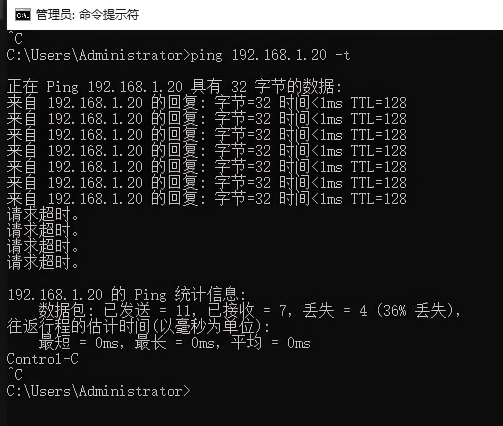
\includegraphics[width=\textwidth]{img/step9/ping_test_failure.png}
        \caption{链路故障时ping丢包现象}
        \label{fig:ping_test_failure}
    \end{subfigure}
    \hfill
    \begin{subfigure}[b]{0.45\textwidth}
        \centering
        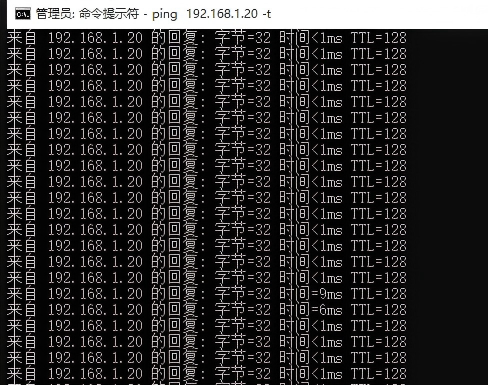
\includegraphics[width=\textwidth]{img/step9/ping_test_recovery.png}
        \caption{故障恢复后ping通信正常}
        \label{fig:ping_test_recovery}
    \end{subfigure}
\end{figure}
丢包分析：故障瞬间丢失4个包（约2秒），收敛后恢复正常通信，无丢包，延迟<1ms。丢包原因是链路切换期间RSTP重新选举根端口和更新转发表。

\subsubsection{故障后生成树信息记录}
\begin{table}[H]
    \centering
    \begin{tabular}{|c|c|c|c|}
        \hline
        属性 & 描述 & 交换机A & 交换机B \\
        \hline
        Port Priority & 网桥优先权 & 128 & 128 \\
        CIST Bridge & 本机网桥ID & 32768.3458-40d7-fee0 & 32768.3458-40d7-f980 \\
        CIST Root/ERPC & 根桥ID/外部路径开销 & 4096.3458-40d7-f980 / 20000 & 4096.3458-40d7-f980 / 20000 \\
        CIST RootPortId & 根端口 & 128.86 (GigabitEthernet0/0/2) & 128.86 (GigabitEthernet0/0/2) \\
        Alternate & 备用端口 & GigabitEthernet0/0/1 & None \\
        \hline
    \end{tabular}
    \caption{交换机生成树信息（故障恢复后）}
\end{table}

对比分析：根端口由G0/0/1变为G0/0/2，交换机A的G0/0/1成为备用端口，两台交换机识别相同根桥和路径开销，网络恢复稳定通信。

\subsubsection{BPDU协议分析}

使用Wireshark捕获BPDU报文：

\begin{figure}[H]
    \centering
    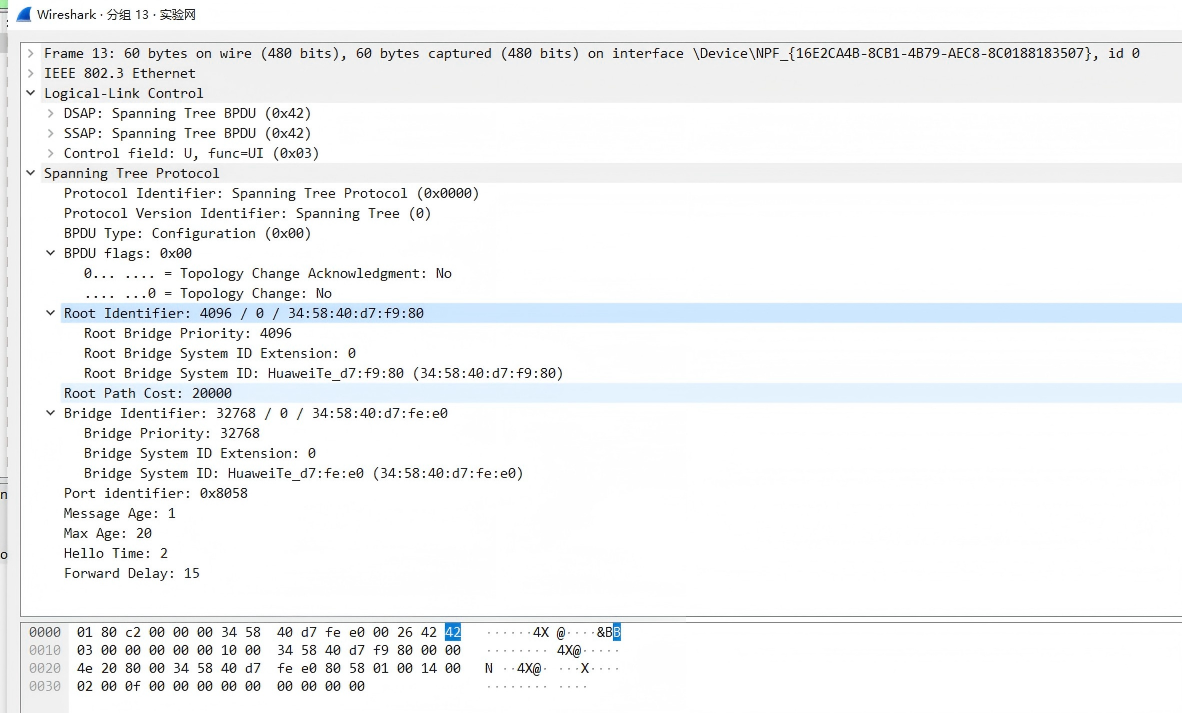
\includegraphics[width=0.7\textwidth]{img/step9/wireshark_bpdu_analysis.png}
    \caption{BPDU报文协议分析}
\end{figure}

BPDU帧结构关键字段：
\begin{itemize}
    \item Root Identifier：4096.34:58:40:d7:f9:80（根桥优先级与MAC）
    \item Bridge Identifier：32768.34:58:40:d7:fe:e0（本桥优先级与MAC）
    \item Hello Time：2秒，Max Age：20秒，Forward Delay：15秒
    \item 路径开销：20000
\end{itemize}

协议作用：BPDU报文定期交换，维护生成树拓扑，根桥信息一致，定时器设置合理，确保网络无环路和快速收敛。

\subsubsection{步骤九小结}
\begin{itemize}
    \item RSTP快速收敛：链路故障后约2秒完成拓扑切换，备用端口成功接替，网络连通性保障。
    \item 丢包可控：故障切换期间仅丢失4个包，随后完全恢复。
    \item 协议机制正确：BPDU报文交换正常，根桥选举、路径计算机制工作正常。
    \item 网络高可用：单链路故障下网络保持稳定通信，冗余设计有效。
    \item 整体评估：RSTP既防环路又快速恢复，实现了高可用性设计目标。
\end{itemize}

\section{实验思考}
\subsection*{(1) 本实验中有无环路？请说明判断理由。如果存在，交换机如何避免环路？}
答：实验网络存在物理环路，但通过生成树协议避免了逻辑环路。
\begin{itemize}
    \item \textbf{判断理由：}
    \begin{itemize}
        \item 拓扑图显示两台交换机通过两条链路互联，形成三角形结构，属于物理环路。
        \item 未启用生成树协议时，广播风暴、端口利用率飙升、MAC地址表震荡等现象均已出现。
    \end{itemize}
    \item \textbf{环路避免机制：}
    \begin{itemize}
        \item 根桥选举：比较桥ID（优先级+MAC），数值小者为根桥。
        \item 端口角色分配：根端口、指定端口转发，备用端口阻塞。
        \item 状态机控制：根端口和指定端口为FORWARDING，备用端口为DISCARDING（逻辑阻塞）。
    \end{itemize}
\end{itemize}

\subsection*{(2) 冗余链路会不会出现MAC地址表不稳定和多帧复制问题？请举例说明。}
答：未启用生成树协议时会出现，启用后不会。可以查看上述实验步骤一和四的对比结果。
\begin{itemize}
    \item \textbf{未启用STP/RSTP：}
    \begin{itemize}
        \item MAC地址表震荡：同一MAC地址在不同端口间频繁切换。
        \item 多帧复制：同一数据帧通过不同路径到达目的设备。
        \item 原因：广播风暴导致数据包在环路中无限循环。
    \end{itemize}
    \item \textbf{启用RSTP后：}
    \begin{itemize}
        \item MAC地址表稳定，学习端口固定。
        \item 无多帧复制，数据沿唯一路径转发。
        \item BPDU统计：阻塞端口仅接收BPDU，不转发数据。
    \end{itemize}
    \item \textbf{结论：} 生成树协议通过逻辑阻塞冗余端口，确保二层转发稳定性。
\end{itemize}

\subsection*{(3) 改用STP协议，重点观察状态转换时间。}
\begin{figure}[H]
    \centering
    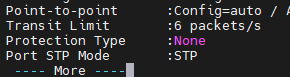
\includegraphics[width=0.7\textwidth]{img/think/stp_mode_configuration.png}
    \caption{STP模式下端口配置信息}
\end{figure}
\begin{itemize}
    \item \textbf{STP收敛机制：}
    \begin{itemize}
        \item 阻塞$\rightarrow$监听：Max Age超时（约20秒）
        \item 监听$\rightarrow$学习：Forward Delay（约15秒）
        \item 学习$\rightarrow$转发：Forward Delay（15秒）
        \item 总收敛时间约50秒
    \end{itemize}
    \item \textbf{RSTP收敛机制：}
    \begin{itemize}
        \item 端口间快速协商，收敛时间1-2秒
    \end{itemize}
    \item \textbf{实验现象对比：}
    \begin{tabular}{|c|c|c|c|}
        \hline
        指标 & STP模式 & RSTP模式 & 差异分析 \\
        \hline
        首次丢包时间 & 故障后20秒 & 故障后立即 & STP需等待Max Age超时 \\
        丢包持续时间 & 30秒 & 1-2秒 & STP需完整状态转换 \\
        总恢复时间 & 50秒 & 2秒 & RSTP快25倍 \\
        \hline
    \end{tabular}
    \item \textbf{工程意义：} STP长时间中断会导致TCP超时、VoIP掉线，RSTP显著提升网络可用性。
\end{itemize}

\subsection*{(4) 两台交换机间多接一根跳线后是否有广播风暴？}
答：是否产生广播风暴取决于是否启用生成树协议。可以对比查看上述实验步骤一和四的结果。
\begin{itemize}
    \item \textbf{未启用生成树协议：}
    \begin{itemize}
        \item 会产生广播风暴，端口利用率100\%，Ping严重丢包。
    \end{itemize}
    \item \textbf{启用RSTP协议：}
    \begin{itemize}
        \item 不会产生广播风暴，网络通信正常，冗余端口被阻塞。
    \end{itemize}
    \item \textbf{技术解析：}
    \begin{itemize}
        \item 广播风暴需物理环路和广播/组播帧同时存在。
        \item 启用RSTP后，物理环路存在但逻辑上阻塞冗余端口，广播帧无法循环，不会风暴。
    \end{itemize}
\end{itemize}

\section{实验总结}
\subsection{主要收获}
\begin{itemize}
    \item 深刻理解了二层网络环路的危害，掌握了广播风暴和MAC地址表震荡的现象与原理。
    \item 熟悉了华为交换机的基本配置流程，包括VLAN、端口类型、端口组等操作。
    \item 掌握了生成树协议（STP/RSTP）的核心机制，包括根桥选举、端口角色分配、路径开销计算等。
    \item 通过实际抓包和端口状态验证，理解了RSTP的快速收敛优势及其对网络高可用性的保障作用。
    \item 学会了使用Wireshark分析BPDU报文，能够定位生成树协议的关键字段和运行状态。
    \item 能够通过优先级配置主动控制根桥选举，提升网络设计的灵活性和可靠性。
\end{itemize}
\subsection{遇到的问题及解决方案}
\begin{itemize}
    \item \textbf{交换机命令不熟悉：} 初次操作华为交换机时，部分命令记忆不牢，参考官方文档和实验指导书逐步完成配置。
    \item \textbf{环路现象定位：} 广播风暴现象初期不易察觉，通过抓包和端口利用率分析，准确定位问题根源。
    \item \textbf{RSTP收敛验证：} 收敛时间测试需精确操作，采用持续ping和端口状态查询，结合丢包现象分析收敛过程。
\end{itemize}
通过本次实验，理论与实践紧密结合，对生成树协议的理解更加深入，网络故障排查和配置能力显著提升，为后续网络课程和实际工程应用打下坚实基础。
\end{document}